\chapter{Decoding of HMMs}

\section{Problems definitions}

\section{The Most Probable Set of States}
\label{sec:set}
\begin{reformulate*}
In this section, we prove NP-hardness of finding the most probable set
of states. Again, as with footprint, this is a special case of the
problem of finding the most probable set of labels. 

\begin{theorem}The following problem is NP-hard:
Given an HMM $H$, sequence $X$ of length $n$, and a number $p\in [0,1]$,
decide if there exists a set of states $S$ such that 
$\Pr\left(s(\pi)=S, X\mid H, n \right)\geq p$.
\end{theorem}\label{thm:sets}

To prove this theorem, we will use a reduction from the maximum clique
problem.  Given a graph $G=(V,E)$ and a clique
size $k$, we first choose a suitable threshold $k'\ge k$, as
detailed below, and construct a graph $G'=(V',E')$ such that $G'$ has
a clique of size $k'$ if and only if $G$ has a clique of size
$k$. This is achieved simply by adding $k'-k$ new vertices and
connecting each of the new vertices to all other vertices in $V'$.
As long as $k'-k$ is not too large, this transformation can be done in
polynomial time.

In the next step, we use $G'$ and $k'$ to construct an HMM, an input
sequence and a probability threshold. We will use the following
straightforward way of converting a graph to an HMM.

\begin{definition}\label{GraphHMM}
Let $G=(V,E)$ be an undirected graph (without self-loops). 
Then the \emph{graph HMM} $H_G$ is defined as follows:
\begin{itemize}
\item Its set of states is $V\cup \{\psi\}$, where $\psi\notin V$ is a
  new state called the error state.
\item Its emission alphabet is $\{0,1\}$.
\item Each state $v\in V$ has initial probability $I(v) = 1/|V|$, the
error state has initial probability $I(\psi)=0$.
\item Each state $v\in V$ emits 0 with probability 1, the error state emits 1 
with probability 1.
\item Transitions with non-zero probability between states $u,v\in V$
  correspond to edges in $E$:
$$a(u,v)=\begin{cases}
\frac1{|V|} & \{u,v\}\in E\\
0 & \text{otherwise}
\end{cases}$$
\item For $u\in V$, we also have $a(u,\psi)=1-\sum_{v\in V}a(u,v)$
and $a(\psi,u)=0$. The error state has a self-transition with 
probability 1: $a(\psi,\psi)=1$.
\end{itemize}
\end{definition}

The error state $\psi$ is added to the HMM so that all non-zero
transitions between states in $V$ have the same probability. Any state
path $\pi$ containing only states from $V$ connected by transitions
with non-zero probability has the same probability of generating
sequence $X=0^n$: $\Pr(\pi, X=0^n|H_G,n) = |V|^{-n}$.
Such paths correspond to walks in graph $G$. 

Therefore, we will be interested in counting the number of walks in
different graphs. Let $Y(n,G)$ be the number of walks of length $n-1$
in a graph $G=(V,E)$ that visit every vertex from $G$ at least once.
Note that a walk of length $n-1$ contains $n-1$ edges and $n$ vertices, and
therefore $Y(n,G)=0$ for $n<|V|$. As a special case we consider
$D(n,k)=Y(n,K_k)$, where $K_k$ is the complete graph with $k$
vertices. The following claim clearly holds:

\begin{lemma}\label{NotCliqueIsSmaller}
If $G$ is a graph with $k$ vertices and $n\ge k$, then
$Y(n,G)\le D(n,k)$ with equality only for $G=K_k$. 
\end{lemma}

In our reduction, we use HMM $H=H_{G'}$ and $X=0^n$ for a suitable
choice of $n$ discussed below. We will set threshold $p$ to
$D(n,k')/|V|^{n}$. Clearly, if the input graph $G$ has a clique $S$ of
size $k$, graph $G'$ has a clique $S'$ of size $k'$. There
are $D(n,k')$ walks of length $n-1$ that use only vertices in
$S'$ and visit each of them at least once. Each such walk
corresponds to one state path, and therefore the probability of
the set of states $S'$ is exactly $p$. 

In order to prove the opposite implication, we need suitable choices
of $n$ and $k'$. Table \ref{DNKTable} shows values of $D(n,k)$ for
small values of $n$ and $k$. For a fixed length of walk $n$, the
number of walks in $K_k$ initially grows with increasing $k$, as we
have more choices which vertex to use next, but as $k$ approaches $n$,
$D(n,k)$  may start to decrease, because the walks are more constrained by
the requirement to cover every vertex. We are particularly interested in
the value of $k$ where $D(n,k)$ achieves the maximum value for a fixed $n$. 
In particular we use the following notation:
$$M_{n} = \min\left\{k ; D(n,k) = \max_{0\leq k'\leq
  n}D(n,k')\right\}$$ Note that if there are multiple values
of $k$ achieving maximum, we take the smallest one as $M_n$.  In our
reduction, we would like to set $n$ to be the smallest value such that
$M_n=k$, but we were not able to prove that such $n$ exists for each $k$.
Therefore we choose as $n$ the smallest value such that $M_n\ge k$, and 
we denote this value $n_k$. As $k'$ we then use $M_{n_k}$. The following 
lemma states important properties of $n_k$ and $M_{n_k}$. 

\end{reformulate*}
\begin{table*}[t]
\begin{center}
\begin{tabular}{|c||c|c|c|c|c|c|c|c|c||c|}\hline
\bf n/k&\bf 0&\bf 1&\bf 2&\bf 3&\bf 4&\bf 5&\bf 6&\bf 7&\bf 8&\bf
$\mathbf{M_n}$\\\hline\hline
\bf 0&{\bf 1}&&&&&&&&&0\\\hline
\bf 1&&\bf 1&&&&&&&&1\\\hline
\bf 2&&&\bf 2&&&&&&&2\\\hline
\bf 3&&&2&\bf 6&&&&&&3\\\hline
\bf 4&&&2&18&\bf 24&&&&&4\\\hline
\bf 5&&&2&42&\bf 144&120&&&&4\\\hline
\bf 6&&&2&90&600&\bf 1200&720&&&5\\\hline
\bf 7&&&2&186&2160&7800&\bf 10800&5040&&6\\\hline
\bf 8&&&2&378&7224&42000&100800&\bf 105840&40320&7\\\hline
\bf 9&&&2&762&23184&204120&756000&\bf 1340640&1128960&7\\\hline
\bf 10&&&2&1530&72600&932400&5004720&13335840&\bf 18627840&8\\
\hline\hline
$\mathbf{n_k}$&0&1&2&3&4&6&7&8&10&\\\hline 
$\mathbf{M_{n_k}}$&0&1&2&3&4&5&6&7&8&\\\hline 
\end{tabular}
\end{center}
\caption{Values of $D(n,k)$, $n_k$, $M_n$, and $M_{n_k}$ for small values of $n$ and $k$. Empty cells contain zeros.}\label{DNKTable}
\end{table*}

\begin{reformulate*}
\begin{lemma}\label{DNKlemma}
The value of $n_k$ is at most $\lceil k\ln k\rceil$, and $n_k$ and
$M_{n_k}$ can be computed in $O(k^{O(1)})$ time.
\end{lemma}

Before proving this lemma, we finish the proof of the reduction. Let
us assume that there is a set of states $S$ such that
$\Pr(s(\pi)=S,X|H,n)\ge p$. This means that if we consider walks in the
subgraph $G'(S)$ induced by the set $S$, we get $Y(n,G'(S))\ge
D(n,k')$. We will consider three cases:
\begin{itemize}
\item If $S$ is a clique and $|S|\ge k'$, we have the desired clique in 
graph $G'$, and therefore there is also a clique of size $k$ in graph $G$. 
\item If $S$ is a clique and $|S|<k'$, then by definition of $M_n$ we have 
$Y(n,G'(S))=D(n,|S|)<D(n,M_n) = 
D(n,k')$. This is a contradiction with our assumption. 
\item If $S$ is not a clique, then by Lemma \ref{NotCliqueIsSmaller}
  and definition of $M_n$ we have $Y(n,G'(S)) < D(n, K_{|S|}) \le
  D(n,M_n) = D(n,k')$. Again we get a contradiction with 
the inequality $Y(n,G'(S))\ge D(n,k')$.
\end{itemize}
Therefore, we have proved that $G$ contains a clique of size $k$ if and
only if the most probable set of states in $H_{G'}$ that can generate $X$ has
probability at least $p$. Moreover, we can construct $n_k$, $M_{n_k}$,
$H_{G'}$, $X$, and $p$ in polynomial time.
To complete this proof we need to prove Lemma \ref{DNKlemma}.  We
start by proving another useful lemma.

\begin{lemma}\label{RecurenceLemma}
The following recurrence holds for $2\leq k\leq n$:
$$D(n,k)=(k-1) D(n-1,k) + k D(n-1,k-1).$$
In addition, $D(n,n)=n!$, $D(n,1) = 0$ for $n>1$, and $D(n,k) = 0$ for $k>n$.
\end{lemma}
\begin{proof}
Clearly, $D(n,n)=n!$ since walks of length $n-1$ correspond to
permutations of vertices.  If $n>1$ then $D(n,1)=0$, since $K_1$ does
not contain any edges.  If $k>n$, $D(n,k)=0$ since a walk of length
$n-1$ can pass through at most $n$ vertices.

Now let $2\leq k\leq n$. Denote as $v(w)$ the number of different
vertices covered by walk $w$. Let $w$ be a walk of length $n-1$ with
$v(w)=k$ and let $w'$ be a walk obtained by taking the first 
$n-1$ vertices of walk $w$. Then $v(w')$ is either $k$ or $k-1$. 

Every walk $w'$ of length $n-2$ with $v(w')=k$ can be extended to a
walk $w$ of length $n-1$ in $K_k$ in $k-1$ ways, because as the last vertex
of $w$ we can use any vertex except the last vertex of $w'$. Therefore
there are $(k-1) D(n-1,k)$ different walks $w$ in $K_k$ with
property $v(w')=k$.

On the other hand if $v(w')=k-1$, we can create a walk $w''$ in
$K_{k-1}$ by renumbering the vertices in $w'$ so that only numbers
$\{1,\dots,k-1\}$ are used (if the vertex missing in $w'$ is $i$, we
replace $j$ by $j-1$ for every vertex $j>i$).  The same
representative $w''$ is shared by $k$ different walks $w$, because to
create $w$ from $w''$, we need to choose the missing vertex $i$ from
all $k$ possibilities, renumber vertices to get $w'$ and then to add
the missing vertex $i$ at the end of the walk. Therefore there are
$kD(n-1,k-1)$ walks with the property $v(w')=k-1$. Combining the two
cases we get the desired recurrence.\qed
\end{proof}

\begin{proof}[Proof of Lemma \ref{DNKlemma}] 
Assume that $k\ge 3$. Clearly, $D(n,k)\leq k(k-1)^{n-1}$, since
$k(k-1)^{n-1}$ is the number of all walks of length $n-1$ in
$K_k$. However, this number includes also walks avoiding some
vertices. The number of such walks can be bounded from above by
$k(k-1)(k-2)^{n-1}$ where we choose one of the $k$ vertices to avoid
and then consider all possible walks on the remaining $k-1$
vertices. In this way we count some walks multiple times; nonetheless
by Bonferroni inequality we obtain bound $D(n,k)\geq
k(k-1)^{n-1}-k(k-1)(k-2)^{n-1}$.

For $k\ge 4$ we therefore have that if
$(k-1)(k-2)^{n-1}<k(k-1)^{n-1}-k(k-1)(k-2)^{n-1}$, then
$D(n,k-1)<D(n,k)$.  By taking logarithm of both sides of the inequality, we
obtain $n>f(k)$ where $f(k) = 1+\frac{\ln(k^2-1)-\ln
  k}{\ln(k-1)-\ln(k-2)}$.  Let $n = \lceil f(k)\rceil$ for some $k\ge
4$ and consider row $n$ in Table \ref{DNKTable}.
We have that $D(n,k-1)<D(n,k)$ and since function $f$ is
increasing, we also we have that $D(n,k'-1)<D(n,k')$ for all $k'\le k$ 
(we have proved it only for $k'\ge 4$, but it is easy to see that it is
also true for $2\le k'\le 3$). The maximum in row $n$ is therefore
achieved at some position $M_n \ge k$. Recall, that $n_k$ is the
smallest $n$ such that $M_n\ge k$. Therefore $n_k\leq \lceil f(k)\rceil$.
The function $k \ln k/f(k)$ is decreasing and its limit is $1$ as $k$
approaches $\infty$. Therefore $\lceil f(k)\rceil\leq\lceil k\ln k\rceil$,
which gives us the inequality $n_k\le \lceil k \ln k\rceil$. This inequality 
can also be easily verified for $k<4$. Since $M_n\le n$,
we also have $M_{n_k}\le \lceil k \ln k\rceil$. 

We can compute $n_k$ and $M_{n_k}$ by filling in table $D(m,j)$ for
all values of $m$ and $j$ up to $\lceil k\ln k\rceil$ using the
recurrence from Lemma \ref{RecurenceLemma}. Since $D(n,k)\leq k^n\leq
n^n$, we can store $D(m,j)$ in $O(k \mbox{polylog}(k))$ bits.
Therefore computing the desired values $n_k$ and $M_{n_k}$ 
can be done in polynomial time. \qed
\end{proof}

%By using the same reduction as in Theorem \ref{thm:sets}, we can
%also prove NP-hardness of the following variant of the problem, in
%which we restrict the size of the set of states $S$. 

%\begin{corollary}
%The following problem is NP-hard:
%Given is an HMM $H$, sequence
%$X$ of length $n$, integer $k$ and a number $p\in [0,1]$ and the task to
%decide if there exists a set of states $S$ of size exactly $k$ 
%such that $\Pr\left(s(\pi)=S, X\mid H, n \right)\geq p$.
%\end{corollary}

%We can easily see that the existence of a clique
%of size $k$ in $G$ leads to the existence of the desired set of states
%$S$ of size exactly $k'$, and by following the reasoning from the
%proof, we can also prove that the converse is true.

Note that it is not clear if the most probable set of states problem is in
NP. In particular, given a set of states $S$, it is NP-hard to find out if its
probability is greater than some threshold $p$, even if this threshold
is 0, as we show next.

\begin{theorem}
Given HMM $H$, sequence $X$ of length $n$ 
and a subset of state space $S$, the problem of deciding if
$\Pr\left(s(\pi)=S, X\mid H, n\right)$ is non-zero is NP-complete.
\end{theorem}

\begin{proof}
Let $G=(V,E)$ be a graph  
and $H_G$ be the corresponding graph HMM as
in Definition \ref{GraphHMM}. Let $X=0^{|V|}$.  
%Any state path
%that can generate $X$ and contains all vertices from $V$ contains each
%vertex exactly once.  
It is easy to see that $\Pr\left(s(\pi)=V,X \mid H_G, |X|
\right)>0$ if and only if $G$ contains a Hamiltonian path. \qed
\end{proof}

Unlike the most probable footprint problem, which was NP-hard even for
a fixed HMM of a constant size, the most probable set problem is
fixed-parameter tractable with respect to the size of the HMM. Given
an HMM with $m$ states and a sequence of length $n$, we can find the
most probable set of states in time $O(2^m m^2 n)$ by a dynamic
programming algorithm similar to the Forward algorithm.
We define $F[i,S,v]$ to be the sum of probabilities of all
states paths $\pi$ of length $i$ such that $s(\pi)=S$, $\pi$ ends in
state $v$ and generates the first $i$ characters of sequence $X$.
To compute $F[n,S,v]$, we use the following equation:
\ifx\settwocolumn\undefined
$$F[i,S,v] = \begin{cases}
I(v)e(v,X[1])& i=1,S=\{v\}\\ 
\displaystyle \sum_{u\to v}a(u,v)e(v,X[i])\left(F[i-1,S\backslash\{v\},u]
+ F[i-1,S,u]\right) & i>1, v\in S\\
0 & \mbox{otherwise}
\end{cases}$$
\else
$$F[i,S,v] = \begin{cases}
I(v)e(v,X[1])& i=1,S=\{v\}\\ 
\displaystyle \sum_{u\to v}a(u,v)e(v,X[i])\\\hspace{5mm}\left(F[i-1,S\backslash\{v\},u]\right.
\\\hspace{5mm}\left.
+ F[i-1,S,u]\right) & i>1, v\in S\\
0 & \mbox{otherwise}
\end{cases}$$
\fi

\end{reformulate*}
\section{Most probable footprint}
\begin{notmytext*}
\label{sec:footprint}

Finding the most probable
footprint is a reasonable decoding criterion,
and it may also serve as a starting point in a multi-stage
strategy. In this section, we show that this problem is
NP-hard. In particular, we will consider the footprint of a state path
$f(\pi)$. The problem of optimizing the footprint of a labeling
$f(\ell(\pi))$ is also NP-hard, because optimizing $f(\pi)$ is its special case, 
equivalent to optimizing $f(\ell(\pi))$ in an HMM in
which each state has a unique label.

\begin{theorem}
There is a fixed HMM $H$ such that the following problem is NP-complete:
Given a sequence $X$ of length $n$ and probability $p\in [0,1]$, determine
if there is a footprint $F$ such that $\Pr(f(\pi)=F,X\mid H,n)\ge p$.
\label{thm:foot}
\end{theorem}

\end{notmytext*}

\begin{figure*}[t]
\centerline{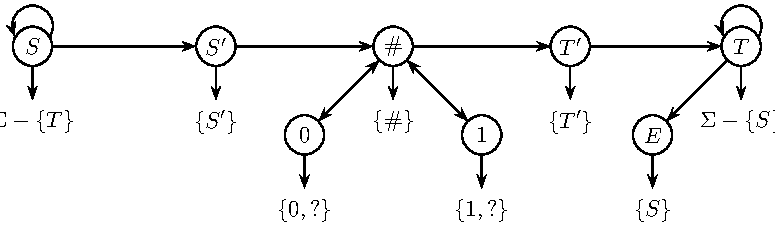
\includegraphics[scale=0.68]{../figures/jcss/cliquehmm.pdf}}
\caption{\label{fig:footprint_hmm} The HMM from the proof of Theorem
  \ref{thm:foot}. States are shown as circles; under each we
  list the set of symbols that the state emits with non-zero
  probability. Each of these symbols is emitted with probability
  $1/k$, where $k$ is the size of the set. The HMM always starts in
  state $S$. All outgoing transitions from a particular state have
  the same probability.}
\end{figure*}
\begin{notmytext*}
\begin{proof}
We will prove NP-hardness by a reduction from the maximum clique problem
using the HMM in Figure 
\ref{fig:footprint_hmm} with eight states and
alphabet $\Sigma=\{S,S',T,T',\#,0,1,?\}$. 


%Popis zakodovania grafu
Let $G=(V,E)$ be an undirected graph with $n$ vertices
$V=\{1,2,\dots,n\}$. We will encode it in a sequence $X$ over alphabet $\Sigma$ as follows.
For every vertex $v\in V$, we create a block $X_v$ with 
$2n+3$ symbols: $X_v=S'\#b_{v,1}\#b_{v,2}\#\dots\#b_{v,n}\#T'$, where $b_{i,j}=1$ 
if $i=j$, $b_{i,j}=?$ if $(i,j)\in E$ and $b_{i,j}=0$ otherwise. 
Sequence $X$ is a concatenation of blocks for all vertices 
with additional first and last symbols: $X=SX_1X_2\dots X_nT$.

All state paths that can generate $X$ have a similar structure. The first
symbol $S$ and several initial blocks are generated in state $S$, one
block, say $X_i$, is generated in states $S'$, $\#$, $0$, $1$, and
$T'$ and the rest of the sequence, including the final symbol $T$, is
generated in state $T$. We will say that a state path with this
structure \emph{covers} the block $X_i$.  Note that state $E$ is never used in
generating $X$, its role is to ensure that the probability of
self-transition is the same in states $S$ and $T$.
All state paths that can generate $X$ have the same
probability $q = \Pr(\pi,X\mid H,|X|) = 2^{-2n^2-2n}3^{-n-1}7^{-2n^2-n+1}$.

%celkovo 2n^2+3n+2 symbolov
%1/2 zacni v S
%kazdy symbol v S a T ma 1/7 emisiu a 1/2 tranziciu do dalsieho
% tych symbolov je 2n^2+n-1
%prechody z S' a T', 0, 1 su 1, tych je n+2
%prechody z # so 1/3, tych je n+1
%emisia v S' a T' a # je 1, tych je n+3
%emisia v 0 a 1 je 1/2, tych je n
%
%spolu teda 1/2^{1 + 2n^2+n-1 + n} * 1/3^{n+1} * 1/7^{2n^2+n-1} 


We say that a state path $\pi$ is a \emph{run} of footprint $F$, if
$\pi$ can generate $X$, and $f(\pi)=F$.
Every footprint that can generate $X$ has the following structure:
$F=SS'\#c_1\#c_2\#\dots\#c_n\#T'T$, where $c_i\in\{0,1\}$. 
The probability of footprint $F$ is $qk$, where $k$ is the number of its runs.
Also note that every run of $F$ covers a different $X_i$, because once $X_i$
is known, the whole path is uniquely determined. 

We will now prove that the graph $G$ has a clique of size at least $k$
if and only if there is a footprint for sequence $X$ with
probability at least $qk$.  First, let $R$ be a clique in $G$ of size
at least $k>0$.  Consider the footprint
$F=SS'\#c_1\#c_2\#\dots\#c_n\#T'T$ where $c_i=1$ if $i\in R$ and $c_i=0$
otherwise. For any $i\in R$, there is a run $\pi_i$ of $F$ that covers
$X_i$. This run will use state 1 for generating each $b_{i,j}$ such
that $j\in R$ and thus both $b_{i,j}\in \{?,1\}$ and $c_j=1$.  For
$j\notin R$ we have $b_{i,j}=0$ and $c_j=0$, thus they will use state
0 in $\pi$. Since there is a different run for every $i\in R$, footprint 
$F$ has at least $k$ runs.

Conversely, let $F$ be a footprint with probability at least $qk>0$
and thus with at least $k$ runs. We will construct a clique of size at
least $k$ as follows. Let $R$ be the set of all vertices $i$ such that
$f$ has a run that covers $X_i$. Clearly the size of $R$ is at least
$k$.  Since $F$ has non-zero probability, it has the form
$SS'\#c_1\#c_2\dots\#c_n\#T'T$ for $c_i\in \{0,1\}$. For all $i\in R$,
$c_i=1$ because the $i$-th block has $b_{i,i}=1$. Therefore for all
$i,j\in R$, we have $b_{i,j}\in \{1,?\}$, which means that $(i,j)\in
E$ or $i=j$. This implies that $R$ is indeed a clique.

To summarize, given graph $G$ and threshold $k$, we can compute in
polynomial time sequence $X$ and threshold $qk$ such that $G$ has a
clique of size at least $k$ if and only if sequence $X$ has a
footprint with probability at least $qk$. This completes our reduction.

The problem is in NP (even if HMM is not fixed, but given on input),
because given an HMM $H$, sequence $X$ and a footprint $F$, we can
compute the probability $\Pr(f(\pi)=F,X\mid H,|X|)$ in polynomial time
by a dynamic programming algorithm which considers all prefixes of
$X$ and all prefixes of $F$. If probability $p$ and parameters of HMMs
are given as rational numbers, we can compute all quantities without
rounding in polynomial number of bits. \qed
\end{proof}

\end{notmytext*}

\subsection{Proof}

\subsection{Most probable set of states}
\begin{reformulate*}
In this section, we prove NP-hardness of finding the most probable set of
states. Again, as with footprint, this is a special case of the problem of
finding the most probable set of labels and it is modification of proof of
theorem \ref{thm:foot}. 


\begin{theorem}The following problem is NP-hard:
Given an HMM $H$, sequence $X$ of length $n$, and a number $p\in [0,1]$,
decide if there exists a set of states $S$ such that 
$\Pr\left(s(\pi)=S, X\mid H, n \right)\geq p$.
\end{theorem}\label{thm:sets}

Let $G=(V,E)$ be an undirected graph with $n$ vertices as in proof of theorem
\ref{thm:foot}. Note that $V = \{1, 2, \dots, n\}$. $G$ will be encoded in
sequence $X$ as in proof if theorem \ref{thm:foot}, but without $\#$ symbols.
Let $X_i$ be the block that represents vertex $i$. Then $X=SX_1\dots X_nT$.

Instead of using one fixed HMM, we expand middle part of the model so that it
generates blocks of length $n+2$ ($n$ vertices and $S', T'$ states). We remove
state $\#$ and expand states $0$ and $1$ into $n$ versions of state $0$ and $1$
denoted $0_v$ and $1_v$ for $v \in V$.  Transitions are from $S'$ to $0_1$ and
$1_1$, from $0_n$ and $1_n$ to $T'$ and for all $i<n$ from $c_i$ to $d_{i+1}$
for $c,d\in \{0, 1\}$ as in figure  \ref{fig:set_hmm2}. 

\end{reformulate*}
\begin{figure*}[t]
\centerline{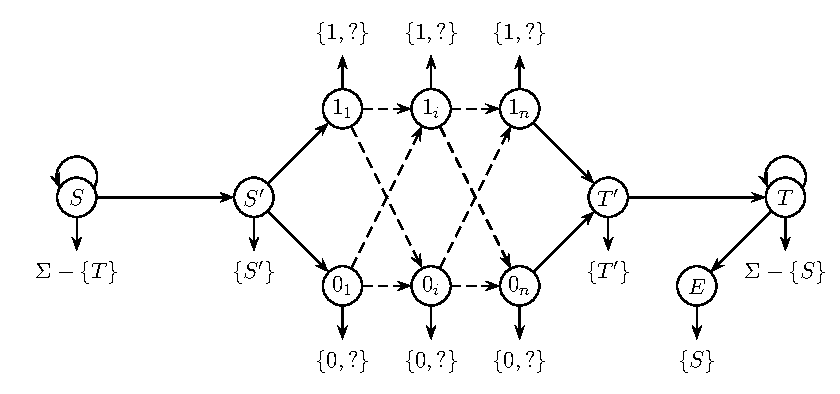
\includegraphics[scale=0.68]{../figures/jcss/expandedcliquehmm.pdf}}
\caption{\label{fig:set_hmm2} The HMM from the proof of Theorem
  \ref{thm:sets}. States are shown as circles; under each we
  list the set of symbols that the state emits with non-zero
  probability. Each of these symbols is emitted with probability
  $1/k$, where $k$ is the size of the set. The HMM always starts in
  state $S$. All outgoing transitions from a particular state have
  the same probability.}
\end{figure*}

\begin{reformulate*}
State paths that generate $X$ have a similar structure as in proof of theorem
\ref{thm:foot}. State $S$ generate the first symbol $S$, some initial blocks,
then one block $X_i$ is generated by some of the states $S', T', 0_v, 1_v, v\in
V$.  Rest of the sequence is generated by terminal state $T$.  Construction of
HMM and sequence $X$ guarantees that for all $v\in V$ exactly one of $0_v, 1_v$
is in the state path. Note that the set of states that is used in such state
path have exactly $n+4$ elements. We say that a state path with this structure
\emph{covers} block $X_i$. All state paths that can generate $X$ have the same
probability $q = \Pr(\pi, X\mid H, |X|) = 2^{-n^2-3n+1}6^{-n^2 - n}$.

We say that a state path $\pi$ is a \emph{run} of set $D$, if $\pi$ can generate
$X$ and $s(\pi) = D$. The probability of set $D$ is $qk$, where $k$ is the
number of runs of $D$. Every run of $S$ covers a different block, since once the
block is known, the path is uniquely determined.

We will now prove that the graph $G$ has a clique of size at least $k$
if and only if there is a set of states for sequence $X$ with
probability at least $qk$.  First, let $R$ be a clique in $G$ of size
at least $k>0$.  Consider the set
$D=\left\{S,S',{c_1},{c_2},\dots,{c_n},T',T\right\}$ where $c_i=1_i$ if $i\in R$
and $c_i=0_i$
otherwise. For any $i\in R$, there is a run $\pi_i$ of $D$ that covers
$X_i$. This run will use state $1_j$ for generating each $b_{i,j}$ such
that $j\in R$ and thus both $b_{i,j}\in \{?,1\}$ and $c_j=1_j$.  For
$j\notin R$ we have $b_{i,j}=0$ and $c_j=0_j$, thus they will use state
$0_j$ in $\pi$. Since there is a different run for every $i\in R$, set 
$D$ has at least $k$ runs.

Conversely, let $D$ be a set of states with probability at least $qk>0$
and thus with at least $k$ runs. We will construct a clique of size at
least $k$ as follows. Let $R$ be the set of all vertices $i$ such that
$D$ has a run that covers $X_i$. Clearly the size of $R$ is at least
$k$.  Since $D$ has non-zero probability, it has the form
$\left\{S,S',c_1,c_2,\dots,c_n,T',T\right\}$ for $c_i\in \{0_i,1_i\}$. For all $i\in R$,
$c_i=1_i$ because the $i$-th block has $b_{i,i}=1$. Therefore for all
$i,j\in R$, we have $b_{i,j}\in \{1,?\}$, which means that $(i,j)\in
E$ or $i=j$. This implies that $R$ is indeed a clique.

Given graph $G$ and threshold $k$, we can compute in
polynomial time sequence $X$ and threshold $qk$ such that $G$ has a
clique of size at least $k$ if and only if sequence $X$ has a
set of states with probability at least $qk$. This completes our reduction.

Note that it is not clear if the most probable set of states problem is in
NP. In particular, given a set of states $S$, it is NP-hard to find out if its
probability is greater than some threshold $p$, even if this threshold
is 0, as we show next.

\begin{theorem}
Given HMM $H$, sequence $X$ of length $n$ 
and a subset of state space $S$, the problem of deciding if
$\Pr\left(s(\pi)=S, X\mid H, n\right)$ is non-zero is NP-complete.
\end{theorem}

\begin{proof} Proof is reduction to problem of finding Hamiltonian path.

\begin{definition}\label{GraphHMM}
Let $G=(V,E)$ be an undirected graph (without self-loops). 
Then the \emph{graph HMM} $H_G$ is defined as follows:
\begin{itemize}
\item Its set of states is $V\cup \{\psi\}$, where $\psi\notin V$ is a
   new state called the error state.
\item Its emission alphabet is $\{0,1\}$.
\ item Each state $v\in V$ has initial probability $I(v) = 1/|V|$, the
error state has initial probability $I(\psi)=0$.
\item Each state $v\in V$ emits 0 with probability 1, the error state emits 1 
with probability 1.
\item Transitions with non-zero probability between states $u,v\in V$
  correspond to edges in $E$:
$$a(u,v)=\begin{cases}
\frac1{|V|} & \{u,v\}\in E\\
0 & \text{otherwise}
\end{cases}$$
\item For $u\in V$, we also have $a(u,\psi)=1-\sum_{v\in V}a(u,v)$
and $a(\psi,u)=0$. The error state has a self-transition with 
probability 1: $a(\psi,\psi)=1$.
\end{itemize}
\end{definition}

The error state $\psi$ is added to the HMM so that all non-zero
transitions between states in $V$ have the same probability. Any state
path $\pi$ containing only states from $V$ connected by transitions
with non-zero probability has the same probability of generating
sequence $X=0^n$: $\Pr(\pi, X=0^n|H_G,n) = |V|^{-n}$.
%Such paths correspond to walks in graph $G$.

Let $G=(V,E)$ be a graph  
and $H_G$ be the corresponding graph HMM as
in Definition \ref{GraphHMM}. Let $X=0^{|V|}$.  
%Any state path
%that can generate $X$ and contains all vertices from $V$ contains each
%vertex exactly once.  
It is easy to see that $\Pr\left(s(\pi)=V,X \mid H_G, |X|
\right)>0$ if and only if $G$ contains a Hamiltonian path. \qed
\end{proof}

Unlike the most probable footprint problem, which was NP-hard even for
a fixed HMM of a constant size, the most probable set problem is
fixed-parameter tractable with respect to the size of the HMM. Given
an HMM with $m$ states and a sequence of length $n$, we can find the
most probable set of states in time $O(2^m m^2 n)$ by a dynamic
programming algorithm similar to the Forward algorithm.
We define $F[i,S,v]$ to be the sum of probabilities of all
states paths $\pi$ of length $i$ such that $s(\pi)=S$, $\pi$ ends in
state $v$ and generates the first $i$ characters of sequence $X$.
To compute $F[n,S,v]$, we use the following equation:
\ifx\settwocolumn\undefined
$$F[i,S,v] = \begin{cases}
I(v)e(v,X[1])& i=1,S=\{v\}\\ 
\displaystyle \sum_{u\to v}a(u,v)e(v,X[i])\left(F[i-1,S\backslash\{v\},u]
+ F[i-1,S,u]\right) & i>1, v\in S\\
0 & \mbox{otherwise}
\end{cases}$$
\else
$$F[i,S,v] = \begin{cases}
I(v)e(v,X[1])& i=1,S=\{v\}\\ 
\displaystyle \sum_{u\to v}a(u,v)e(v,X[i])\\\hspace{5mm}\left(F[i-1,S\backslash\{v\},u]\right.
\\\hspace{5mm}\left.
+ F[i-1,S,u]\right) & i>1, v\in S\\
0 & \mbox{otherwise}
\end{cases}$$
\fi


\end{reformulate*}


\section{The Most Probable State Restriction}

\begin{reformulate*}
\label{sec:restriction}

In the most probable set problem, we consider only paths that use each
state in the set. In some situations, it is more natural to allow
paths to use only some of these states, as in the most probable
restriction problem. However, the set of all states is
trivially the most probable restriction. To get a meaningful problem
definition, we restrict the size of the restriction to be $k$. As we
will show, this problem is also NP-hard.

\begin{theorem}
The following problem is NP-complete: Given is an HMM $H$, sequence
$X$, integer $k$ and number $p\in [0,1]$. Determine if
there is a subset of states $S$ of size $k$ such that 
$\Pr(s(\pi)\subseteq S, X\mid H,|X|)\ge p$. 
\end{theorem}

\begin{proof}
We will prove NP-hardness by a reduction from 3-SAT. Consider an
instance of 3-SAT with the set of variables $U=\{u_1,u_2,\dots,u_n\}$
and the set of clauses $C=\{c_1,c_2,\dots,c_m\}$. 
Based on sets $U$ and $C$, we construct an HMM $H$ as
follows.  The set of states $V$ will contain all positive and negative
literals. The emission alphabet $\Sigma$ contains all clauses, all
variables and a special error symbol $\psi$. The initial probability
of each state is $1/(2n)$, and the transition probability
between any two states is also $1/(2n)$. State for a literal
$u$ emits with probability $1/|\Sigma|$ every clause that contains $u$.
State for literal $u$ also generates the positive form of the literal
with probability $1/|\Sigma|$. For proper normalization, 
it also generates the error symbol 
with probability $1-\sum_{x\in C\cup U}e(v,x)$. 

We also create string $X=u_1u_2\dots
u_nc_1c_2\dots c_m$ and set the size of the restriction $k$ to equal
the number of variables $n$. Every state path $\pi$ that can generate
$X$ has probability $(2n|\Sigma|)^{-|X|}$; we set threshold $p$ to
this value. Each 
variable $u_i$ in the first part of $X$ 
can be generated only by states $u_i$ and
$\bar{u_i}$; therefore one of these states needs to be in the
path. The first portion of the path thus traverses $k$ 
different states; only these states can be used to emit the second part of the
sequence. 
%Every clause can be emitted only by states for literals that
%satisfy it. 
The set of states used by a state path with
non-zero probability therefore corresponds to a satisfying assignment
in a straightforward way. 
%The HMM has a restriction of size $k$ with
%probability at least $p$ if and only if the 3-SAT instance has a
%satisfying assignment.

Note that given a restriction $S$, we can easily verify if its
probability is at least $p$ by a variant of the Forward algorithm
in which we allow only states in $S$. Therefore the problem is in NP.
\qed
\end{proof}
\end{reformulate*}

\section{Decoding of Pair-HMM}

\notmytext{
Tu treba aj nejake veci podokazovat}
\reformulate{Tu treba aj nejake veci podokazovat}
\begin{reformulate*}
Tento text by sa mal asi reformulovat
\end{reformulate*}

\begin{notmytext*}
Intuitivne: Ked sa pohnem k parovym, tak vsetko ostane aspon rovnako tazke, ale mozno budem vediet znizit pocet stavov.
Pravdepodobne intuitivne budem vediet prekladat do znizenia poctu stavov -- v
druhej sekvencii by som mohol nejako kodovat stavy HMM s tym, ze by bola mozno
iba ciastocne vacsia
\end{notmytext*}
